\section*{Log ud}
Log ud inddeles i en boundary og en dertilhørende controller, som det fremgår af \autoref{fig:MVCLogUd}. 

\begin{figure} [H]
\centering
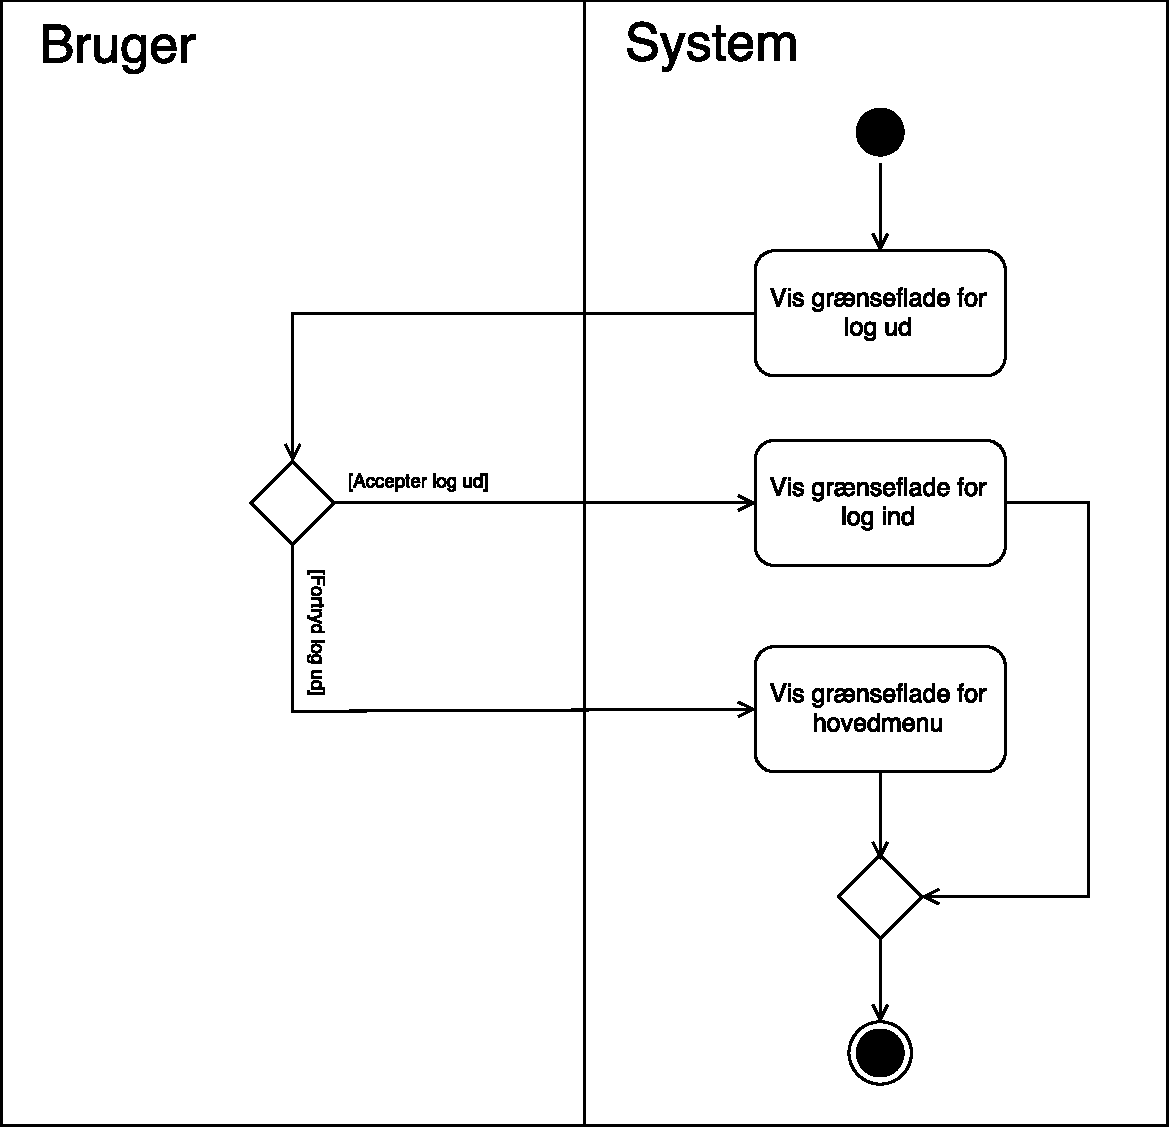
\includegraphics[width=0.6\textwidth]{figures/MVC/Logud}
\caption{Designklasser for log ud. Til venstre ses boundary og til højre controller.}
\label{fig:MVCLogUd}
\end{figure}

\noindent
Der opstilles i \textit{LogudGrænseflade} et tekstfelt, af typen TextView, for log ud. Dertil opstilles en OKKnap og FortrydKnap af typen Button. 
Den tilhørende controller indeholder metoderne, Lyt, Vis, Nulstil, Gem og Start. I sammenspil med designklasserne er der opstillet et sekvensdiagram, som fremgår af \autoref{fig:SEKlogUd}.

\begin{figure} [H]
\centering
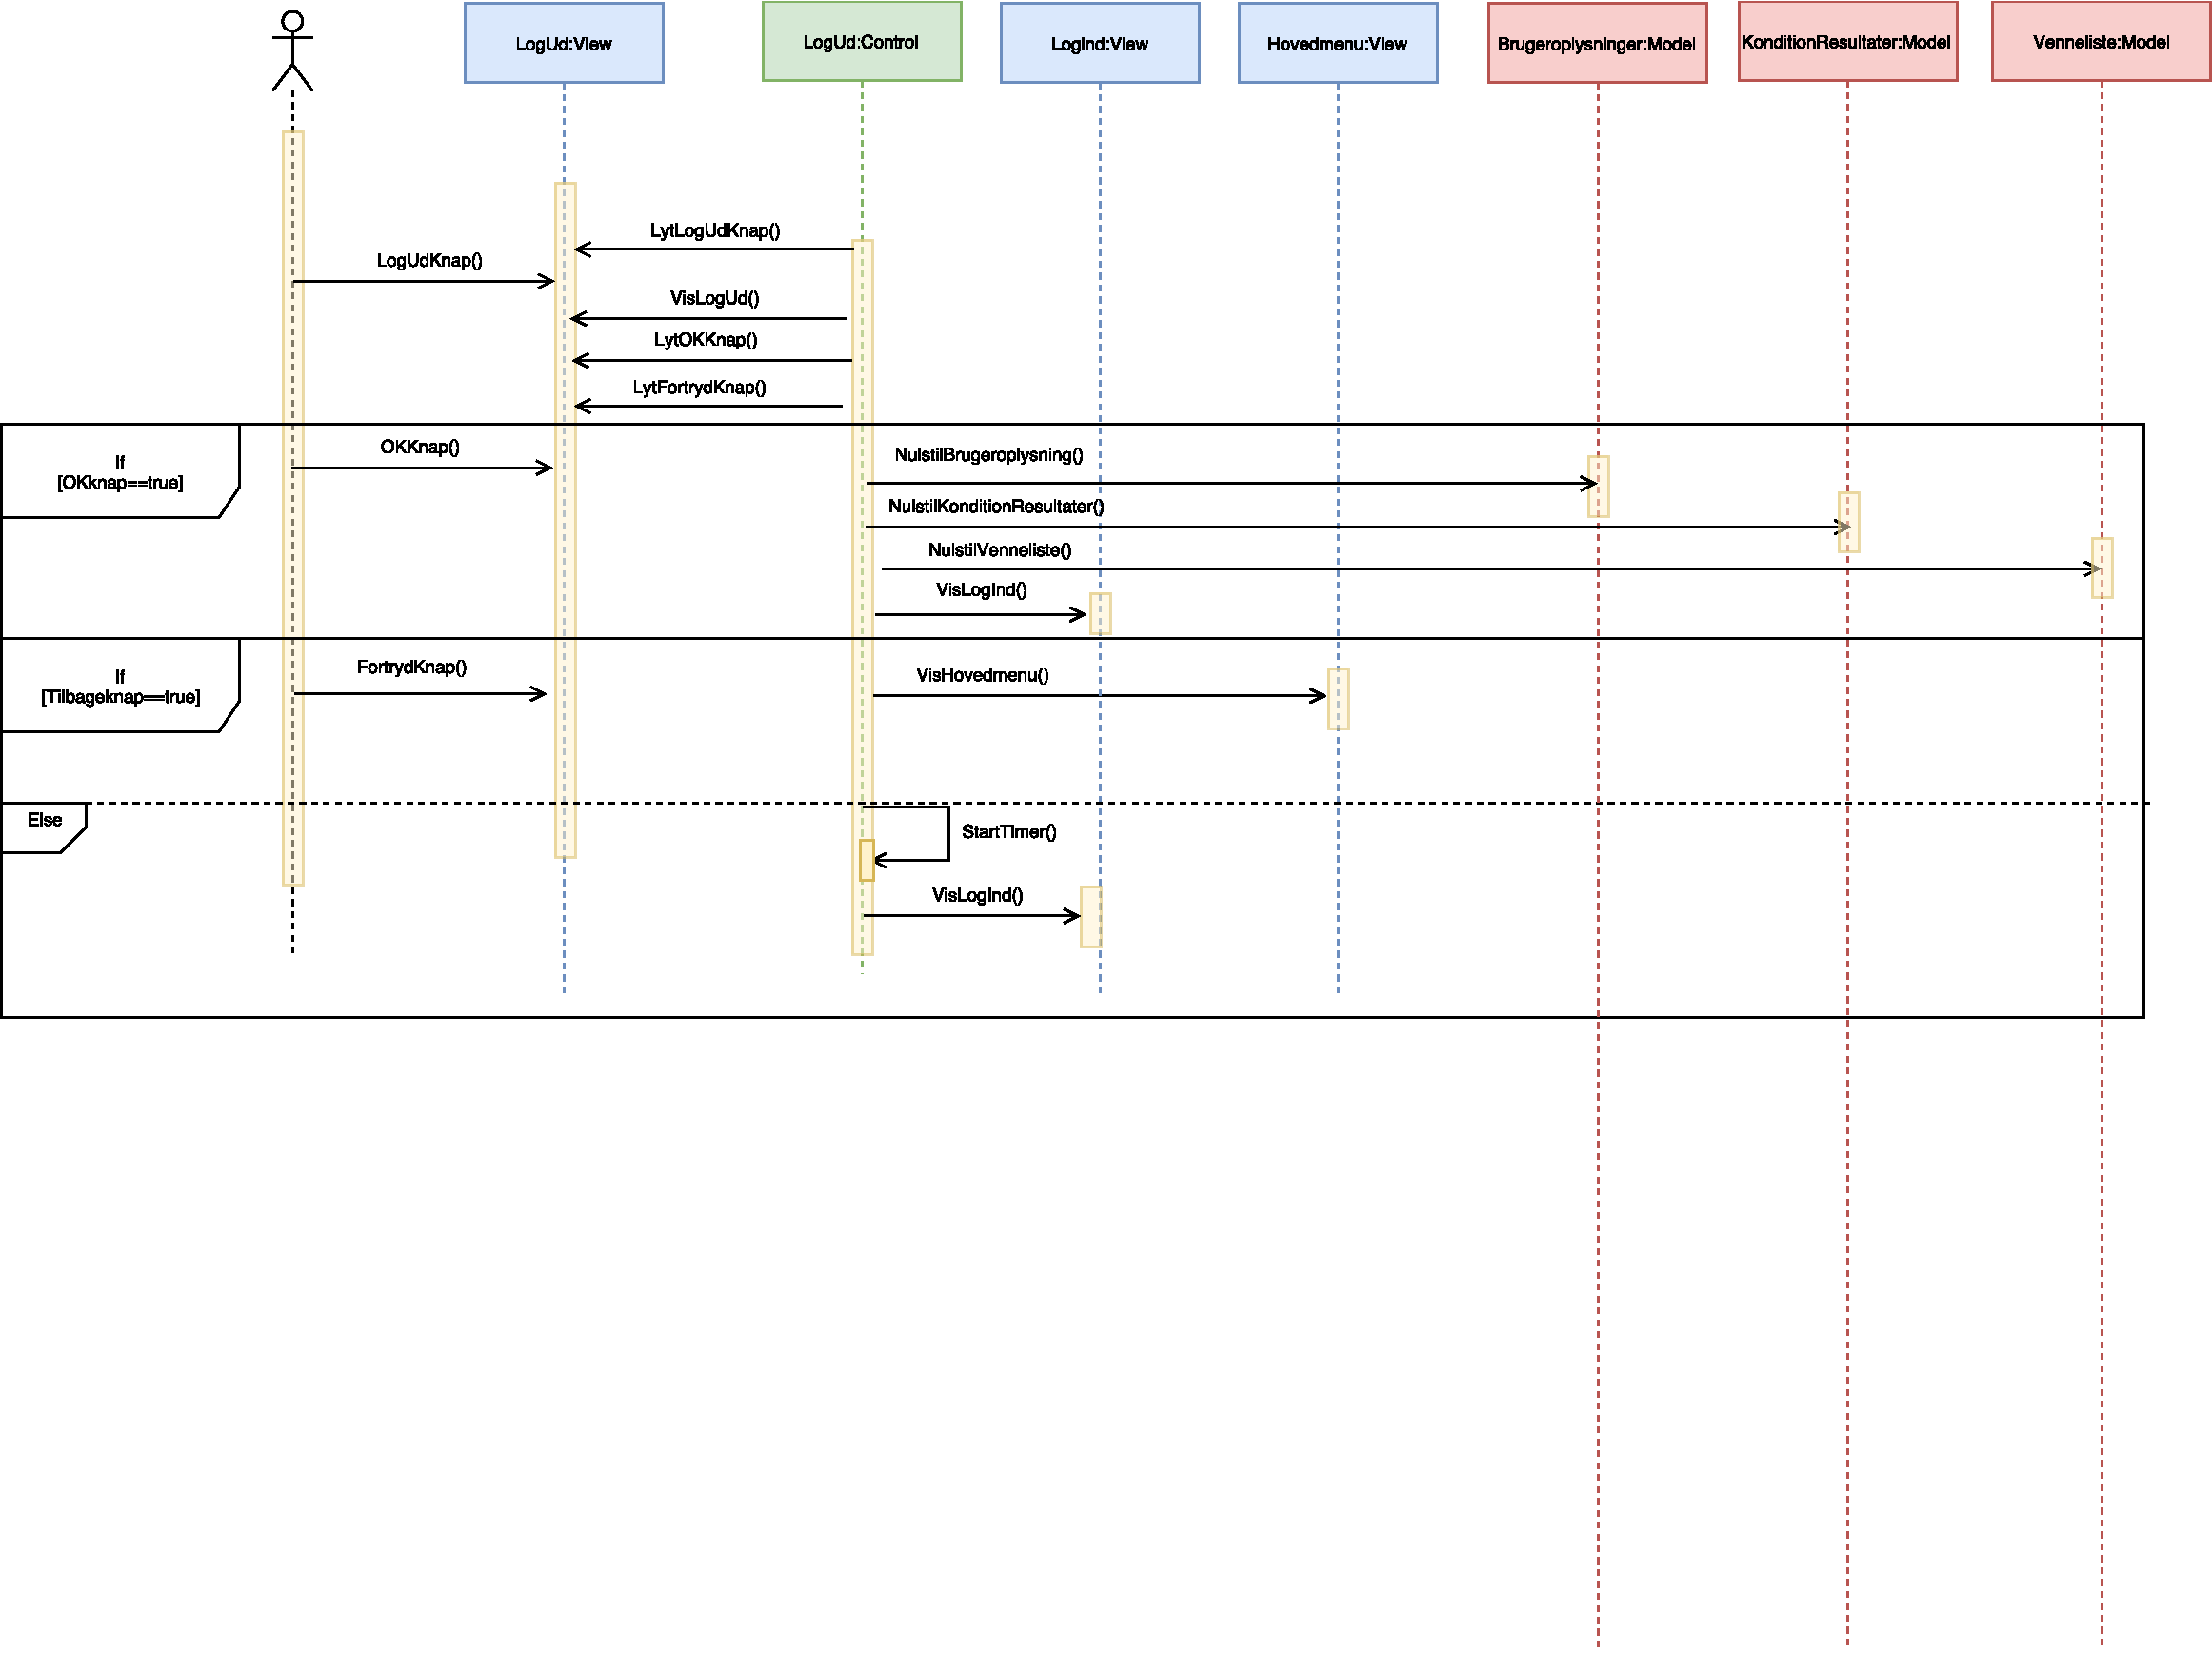
\includegraphics[width=1.1\textwidth]{figures/Sek/SEKLogUd}
\caption{Sekvensdiagram for log ud.}
\label{fig:SEKlogUd}
\end{figure}

\noindent
Når brugeren via grænsefladen for hovedmenuen


Der er til \textit{LogudGrænseflade} opstillet en \textit{LogudController}, der har til formål at lytte til OK eller tilbage knap. Hvis brugeren trykker på OK knappen afsluttet forbindelse til databasen og skærmen for log ind vises. Hvis brugeren trykker på tilbage knappen vises hovedmenuen. Glemmer brugeren at logge ud startes en timer derved inaktivitet i længere tid logger brugeren ud. 